\chapter{Estimators: Bias, Variance and Risk}
\label{ch:estimators}

\begin{chaptergoals}
\begin{itemize}[nosep]
\item What a statistic is, what an estimator is, and the sense in which a statistic throws information away (and when, by the sufficiency principle, that's fine).
\item The two large-sample properties an estimator should have: consistency (it gets to the truth) and asymptotic normality (it gets there at rate $1/\sqrt{n}$ with a Gaussian error), and why the asymptotic variance is not the limit of the variance.
\item The two finite-sample measures: bias and variance, with Jensen's inequality as the reason transformed estimators pick up bias.
\item Quadratic risk $=$ variance $+$ bias$^2$, and the trade-off it makes visible: a biased estimator can beat an unbiased one, and no estimator wins for every value of the parameter.
\end{itemize}
The running example is again the kiss experiment, $R_1, \ldots, R_n \iid \Bern(p)$ with $n = 124$, now with several competing estimators of $p$.
\Cref{ch:models} fixed the object inside which inference happens, and Part II supplied the three limit facts about averages; the first task inside the model is to guess $\theta$ from the data, and this chapter says what a guess is and how to judge one.
\end{chaptergoals}

\section{Statistics and estimators}
\label{sec:est-statistics}

\begin{definition}[Statistic, estimator]
\label{def:estimator}
A \textbf{statistic} is any measurable function of the sample: $T = T(\Xton)$.
For example, $\bar{X}_n$, $\max_i X_i$, $X_1 + \log(1 + \abs{X_n})$, the sample variance, and so on.
As a statistic is a function of your data, it's an r.v.

An \textbf{estimator} of $\theta$ is a statistic $\ethn = \ethn(\Xton)$ whose expression doesn't depend on $\theta$.
\end{definition}

\begin{inwords}
\textbf{In words.} A statistic is anything you can compute from the data. An estimator is a statistic you intend as a guess for $\theta$, and its formula may use the data and known constants only, never $\theta$.
\par\smallskip
\textbf{For the kiss data.} $\bar{R}_n$ is a statistic and an estimator of $p$. $\bar{R}_n - p$ is a random variable but not a statistic, since you cannot compute it. $\max_i R_i$ is a statistic (it is $1$ unless every couple turned left) and a useless estimator of $p$.
\end{inwords}

The word `measurable' is a technicality from probability theory \toolkit{sec:math-rv}; the working rule of thumb is that if you can compute it exactly once you're given the data, it's measurable.
Things that are only implicitly defined, such as a $\sup$ or $\inf$ over an infinite family \toolkit{sec:math-sup}, can fail the condition, but every statistic this book writes down is a formula in the observations and passes it.

The clause `doesn't depend on $\theta$' is the whole content of the second definition.
$\bar{R}_n$ is an estimator of $p$ in the kiss model; $\bar{R}_n - p$ is neither a statistic nor an estimator because you can't compute it from the data alone: its formula involves the thing you're trying to estimate. (It is a perfectly good random variable, and it has a name, the \textbf{estimation error}, which is the quantity the rest of this chapter measures.)
The constant $0.5$ is an estimator of $p$ (a bad one, as \cref{sec:est-strengths} will show), and so is $X_1$: the definition says what an estimator is, not what a good one is.
The rest of the chapter is about telling them apart.

Recall from \cref{ch:kiss} the distinction between an estimator and an estimate: the estimator $\ethn$ is a random variable, with a distribution, an expectation and a variance; the \textit{estimate} $\hat{\theta}_n(x_1, \ldots, x_n)$ is the number it produces on your one sample.
Every property defined in this chapter is a property of the random variable.

\section{A statistic reduces the data}
\label{sec:est-reduction}

Let $\matx = (\Xton)$ be the vector of observations and $\vecx = (x_1, \ldots, x_n)$ a realized sample.
Any statistic $T(\matx)$ defines a form of data reduction.
Anyone who uses only the observed value of the statistic, $T(\vecx)$, rather than the entire observed sample $\vecx$, will treat as equal two samples, $\vecx$ and $\vecy$, that satisfy $T(\vecx) = T(\vecy)$ even though the actual sample values may differ.

Data reduction in terms of a particular statistic can be thought of as a partition of the sample space $E^n$.
For illustration, suppose a sample of size $n$ is drawn and $\bar{x} = 8$.
There are many points in $E^n$ which have the same mean of $8$, and you can think of them as belonging to the set $\{ (x_1, \ldots, x_n) : \bar{x} = 8 \}$.
In fact, all points on the hyperplane
\[
x_1 + \cdots + x_n = 8n
\]
yield the mean $\bar{x} = 8$, and thus the hyperplane is the set.
But there are of course many values that $\bar{X}_n$ can take, and thus there are many such sets.
In this sense, the sample mean, or any statistic, partitions the sample space into a collection of sets (equivalence classes).
\Cref{fig:partition} draws this for $n = 2$, where the sample space is the plane and the hyperplanes are lines, next to the quite different partition induced by the maximum.
On the left, the samples $(1.5, 4.5)$ and $(4.5, 1.5)$ lie on the same line and are the same sample to anyone who only sees $\bar{x} = 3$.
On the right, the level sets of the maximum are L-shapes, and $(1.5, 4.5)$ and $(4.5, 4.5)$ are the same sample to anyone who only sees $\max = 4.5$.
Each statistic keeps one number and discards the rest, and which rest is discarded depends on the statistic.

\begin{figure}[htbp]
\centering
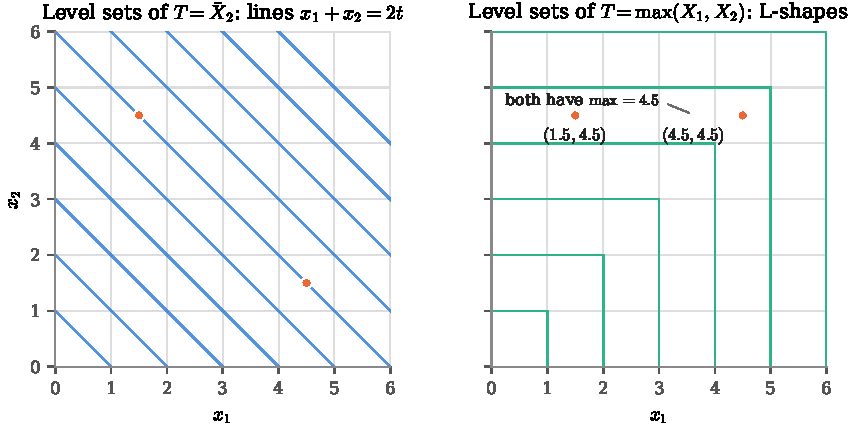
\includegraphics[width=\textwidth]{fig_statistic_partition}
\caption{Level sets of the sample mean (left, the lines $x_1 + x_2 = 2t$) and of the maximum (right, L-shapes) for a sample of size $n = 2$, a point in the plane. Orange dots mark two samples on one level set.}
\label{fig:partition}
\end{figure}

Let $\mathcal{T} = \{ t = T(\vecx) \text{ for some } \vecx \in E^n \}$ be the image of $E^n$ under $T$;
that is, $\mathcal{T}$ is the set of all possible values of the statistic.
Then $T$ partitions the sample space into the sets $A_t = \{ \vecx : T(\vecx) = t \}$ for $t \in \mathcal{T}$.
Samples $\vecx_1$ and $\vecx_2$ belong to the same set if and only if $T(\vecx_1) = T(\vecx_2)$.
The statistic summarizes the data in that, rather than reporting the entire sample $\vecx$, it reports only that $T(\vecx) = t$ or, equivalently, $\vecx \in A_t$.

\subsection{The sufficiency principle}

A \textbf{sufficient statistic} for a parameter $\theta$ is a statistic that, in a certain sense, captures all the information about $\theta$ contained in the sample.
Any additional information in the sample, besides the value of the sufficient statistic, does not contain any more information about $\theta$.
This leads to the data reduction technique called the sufficiency principle.

\textbf{Sufficiency principle:} If $T(\matx)$ is a sufficient statistic for $\theta$, then any inference about $\theta$ should depend on the sample $\matx$ only through the value $T(\matx)$.
That is, if $\vecx$ and $\vecy$ are two sample points such that $T(\vecx) = T(\vecy)$, then the inference about $\theta$ should be the same whether $\matx = \vecx$ or $\matx = \vecy$ is observed.

\begin{definition}[Sufficient statistic]
\label{def:sufficient}
A statistic $T(\matx)$ is a \textbf{sufficient statistic for} $\theta$ if the conditional distribution of the sample $\matx$ given the value of $T(\matx)$ does not depend on $\theta$.
\end{definition}

\begin{inwords}
\textbf{In words.} Once you know the value of $T$, the rest of the sample looks the same whatever $\theta$ is, so the rest carries no further information about $\theta$.
\par\smallskip
\textbf{For the kiss data.} Given that $80$ of $124$ couples turned right, every ordering of the $80$ ones and $44$ zeros is equally likely, whatever $p$ is; the count is sufficient and the order tells you nothing more about $p$. The example below does the computation.
\end{inwords}

\begin{example}
\label{ex:sufficient-bernoulli}
In the kiss model, the number of couples turning right $S = \sum_i R_i$ is sufficient for $p$.
Given $S = s$, every arrangement of $s$ ones and $n - s$ zeros is equally likely:
\[
\Pr_p(\matx = \vecx \mid S = s) = \frac{p^s (1-p)^{n-s}}{\binom{n}{s} p^s (1-p)^{n-s}} = \frac{1}{\binom{n}{s}},
\]
which doesn't involve $p$.
Once you know $80$ of $124$ couples turned right, the order in which they did so tells you nothing further about $p$.
This is why every method in this book for this model is a function of $\bar{R}_n$ alone: by the sufficiency principle, nothing else in the sample tells you more about $p$, if the model is right. (The order of the $R_i$ is exactly what you would look at to check whether it is, as with the wedding reception of exercise 4(b) in \cref{ch:kiss}, whose couples would show up as a run of $1$s.)
\end{example}

Sufficiency has a large theory of its own, which this book does not take up; it appears once more, in \cref{ch:exp-families}, where the exponential families make the sufficient statistic visible.
It is here because it says precisely what the data reduction in \cref{fig:partition} is allowed to throw away: everything except $T$, whenever the conditional distribution of the sample given $T$ is free of $\theta$.

\section{Consistency}
\label{sec:est-consistency}

The best estimator would be the one that equals the parameter of interest.
Given the probabilistic nature of statistics, ascertaining rules to derive such an estimator is hopeless.
But there are desirable properties you want estimators to have.

For example, as you collect more and more data you should get a better and better idea of which distribution generated the data.
In the limit, as your sample size increases to infinity you should know exactly which distribution it is.
Specifically, you want an estimator that converges to the true parameter $\theta$ as your sample size goes to infinity.
An estimator satisfying this property is called \textit{consistent}, and it comes in two forms, depending on whether the convergence is in probability or almost surely.

\begin{definition}[Consistency]
\label{def:consistent}
An estimator $\ethn$ of $\theta$ is \textbf{weakly consistent} if
\[
\ethn \convp \theta \quad (\text{with respect to } \Pr_\theta),
\]
that is, $\Pr_\theta \left( \abs{\ethn - \theta} \geq \epsilon \right) \to 0$ for every $\epsilon > 0$, and \textbf{strongly consistent} if $\ethn \convas \theta$ (almost sure convergence is defined in \cref{app:modes}; the unqualified word `consistent' is used for either, in this book and in common usage).
Here $\Pr_\theta$ is the distribution that generated the data, and the statement is required to hold for every $\theta \in \Theta$.
\end{definition}

\begin{inwords}
\textbf{In words.} With enough data the estimator lands as close to the truth as you like, with probability as high as you like, and this must be so whichever value the truth has.
\par\smallskip
\textbf{For the kiss data.} $\bar{R}_n \convp p$ is the Law of Large Numbers, so $\bar{R}_n$ is consistent. The constant estimator $0.5$ is not: it never moves, so it only gets close to $p$ if $p$ happens to be $0.5$, and consistency has to hold for every $p$.
\end{inwords}

The Law of Large Numbers is the consistency of $\bar{X}_n$ for $\mu$; its weak form (\cref{thm:wlln}) gives weak consistency, its strong form (\cref{thm:slln} in \cref{app:modes}) strong consistency.
\recall{The Law of Large Numbers says that an average of independent draws settles on the number it is an average of: for any width you name, the probability that $\bar{X}_n$ sits outside a band of that width around $\mu$ goes to zero. It says nothing about how fast, and nothing about the shape of what is left; those are the Central Limit Theorem's business.}
The continuous mapping theorem (\cref{ch:limit-tools}) then makes any continuous function of a consistent estimator consistent for the corresponding function of the parameter.
\recall{The continuous mapping theorem says that applying a continuous function to a converging sequence gives a converging sequence, with the function applied to the limit: if $\hat\theta_n \convp \theta$ and $g$ is continuous at $\theta$, then $g(\hat\theta_n) \convp g(\theta)$. It is the rule that lets you take square roots and reciprocals of estimators without starting over.}

Consistency only takes a stand on where the distribution of $\ethn$ \textit{concentrates}, not on the whole distribution.
This is evident from its definition; consistency is defined in terms of convergence in probability or almost surely, and both are statements about the limit being a point.
But consistency usually isn't enough to do inference because you want to know not just where the estimator concentrates but also the precision with which it concentrates, and how fast.

\begin{example}[How fast is consistent?]
\label{ex:rate}
Let $\Xton \iid \Bern(p)$.
What is the smallest $c$ such that $n^c(\bar{X}_n - p)$ does \textit{not} converge to $0$ in probability?
By the CLT, $\sqrt{n}(\bar{X}_n - p)/\sigma \convd \Gauss(0,1)$ with $\sigma = \sqrt{p(1-p)}$, so for $c < 1/2$,
\[
n^c (\bar{X}_n - p) = \frac{\sigma}{n^{1/2 - c}} \cdot \frac{\sqrt{n}}{\sigma} (\bar{X}_n - p) \convd 0 \cdot \Gauss(0,1) = 0
\]
by Slutsky, which is convergence in probability to $0$ since the limit is a constant.
At $c = 1/2$ the limit is $\Gauss(0, \sigma^2)$, not $0$.
So $c = 1/2$: the estimation error $\bar{X}_n - p$ is of exact order $1/\sqrt{n}$, and such an estimator is called \textit{$\sqrt{n}$-consistent}.
That is more than consistency says, and it's the second property.
\end{example}

\section{Asymptotic normality}
\label{sec:est-asymptotic-normality}

This is where the property of asymptotic normality enters, which unlike consistency is \textit{defined in terms of convergence in distribution}.
Asymptotic normality is a property of an estimator that, if present, gives it CLT-like behavior: a Gaussian limiting distribution.
Unlike the CLT, it's not a theorem; it's a property that a given estimator may or may not have, and specifically a property of estimators, hence concerned with inference.
For reasons addressed below, it involves some scaling in order to circumvent a problem with the variance of the limiting distribution.

\begin{definition}[Asymptotic normality]
\label{def:asymp-normal}
An estimator $\ethn$ of $\theta$ is \textbf{asymptotically normal} if
\[
\sqrt{n}(\ethn - \theta) \convd \Gauss(0, \sigma^2).
\]
The variance of this limiting distribution, $\sigma^2$, is called the \textbf{asymptotic variance} of $\ethn$.
\end{definition}

\begin{inwords}
\textbf{In words.} Magnify the estimation error by $\sqrt{n}$ and it settles into a bell curve centered at $0$. Unmagnified, the error is approximately $\Gauss(0, \sigma^2/n)$: shrinking like $1/\sqrt{n}$, with a known shape.
\par\smallskip
\textbf{For the kiss data.} $\sqrt{n}(\bar{R}_n - p) \convd \Gauss(0, p(1-p))$ by the CLT, so $\bar{R}_n$ is asymptotically normal with asymptotic variance $p(1-p) = 0.229$ at $p = 0.645$, and its error at $n = 124$ is approximately $\Gauss(0, 0.043^2)$.
\end{inwords}

\textbf{NB$_1$:} You might imagine the `natural' form of the asymptotic variance would simply be the limit of $\var(\ethn)$ as $n$ goes to infinity.
\textbf{This is not what it is.}
Why not?
Think about the estimator $\bar{X}_n$.
Its variance is $\var(\bar{X}_n) = \sigma^2/n$, and hence, as $n \to \infty$, it converges to 0.
It'd be silly to let `asymptotic variance' refer to something that's always 0.
Hence, the asymptotic variance $\sigma^2$ is \textit{not} the limit of the variance of $\ethn$.
\Cref{fig:asympvar} shows the two quantities side by side for the kiss estimator.
On the left, $\var(\hat{p}) = p(1-p)/n$ goes to zero, and its limit carries no information about precision.
On the right, $n \cdot \var(\hat{p}) = p(1-p) = 0.229$ is constant, and that constant is the asymptotic variance, the variance of the limiting Gaussian of $\sqrt{n}(\hat{p} - p)$.

\begin{figure}[htbp]
\centering
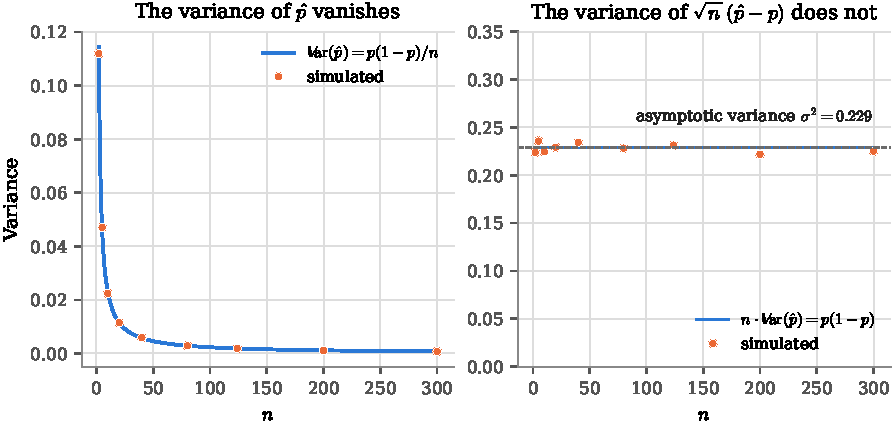
\includegraphics[width=\textwidth]{fig_asymptotic_variance}
\caption{For $\hat{p} = \bar{R}_n$ with $p = 0.645$, against $n$. Left: $\var(\hat{p}) = p(1-p)/n$. Right: $n \cdot \var(\hat{p})$, with the asymptotic variance as a gray dashed line. Blue curves are exact; orange dots are variances estimated from $4{,}000$ simulated samples at each $n$.}
\label{fig:asympvar}
\end{figure}

\textbf{NB$_2$:} This brings us to the rescaling in the definition of asymptotic normality.
The rescaling by $\sqrt{n}$ is crucial because it holds the \textit{spread} of the error fixed as the sample size increases, which is what allows a non-degenerate Gaussian limit to exist at all.
To understand why, again think about $\bar{X}_n$: without the rescaling, $\bar{X}_n - \mu$ converges to the degenerate distribution at $0$, which is consistency restated and says nothing about precision.
With it, $\sqrt{n}(\bar{X}_n - \mu)$ has variance $\sigma^2$ for every $n$ and a Gaussian limit.
For the sample mean the asymptotic variance therefore coincides with $n \var(\bar{X}_n)$; in general it is defined as the variance of the limiting Gaussian, which is the only definition that always makes sense, since convergence in distribution does not by itself say anything about variances.
This is the two-scales picture of \cref{sec:conv-two-scales}, and \cref{ex:rate} says why $\sqrt{n}$ and not some other power.

\textbf{NB$_3$:} Note also that you subtract the unknown parameter $\theta$ from $\ethn$ in the definition.
This focuses attention on the deviation of the estimator from its true value, $\ethn - \theta$, which is the estimation error, the quantity you actually care about.

\begin{intuition}[what asymptotic normality buys]
For large $n$ the error of an asymptotically normal estimator is approximately $\Gauss(0, \sigma^2/n)$.
That one sentence gives you a standard error, $\sigma/\sqrt{n}$; an error bar, $\ethn \pm 1.96 \sigma/\sqrt{n}$ with probability about $95\%$; and a test of any hypothesis about $\theta$.
Consistency says the error vanishes; asymptotic normality says how big it is at the $n$ you have and what shape it has.
\Cref{ch:confidence-intervals} is entirely about using the sentence.
When the asymptotic variance depends on $\theta$ (as $p(1-p)$ does), you'll replace it by a consistent estimate and lean on Slutsky, as in \cref{ch:limit-tools}.
\end{intuition}

\section{Bias}
\label{sec:est-bias}

Consistency and asymptotic normality are properties of the limit.
The next two are properties of $\ethn$ at the sample size you actually have.

\begin{definition}[Bias]
\label{def:bias}
The \textbf{bias} of an estimator $\ethn$ of $\theta$ is
\[
\Bias(\ethn) = \E_\theta[\ethn] - \theta.
\]
If $\Bias(\ethn) = 0$ for every $\theta \in \Theta$, the estimator is called \textbf{unbiased}.
\end{definition}

\begin{inwords}
\textbf{In words.} Average the estimator over all the samples you could have drawn; the bias is how far that average sits from the truth.
\par\smallskip
\textbf{For the kiss data.} $\E[\bar{R}_n] = p$, so $\bar{R}_n$ is unbiased; the constant $0.5$ has bias $0.5 - p$, which is $-0.145$ if $p = 0.645$.
\end{inwords}

An unbiased estimator is right on average: if you could repeat the experiment many times, the estimates would be scattered around $\theta$ with no systematic lean.
It says nothing about how widely they're scattered.

\begin{worked}[four estimators of $p$: bias]
Let $\Xton \iid \Bern(p)$ and consider four candidate estimators of $p$, the first three of which look respectable and the fourth of which does not.
\begin{enumerate}[nosep]
\item $\hat{p} = \bar{X}_n$: $\E[\bar{X}_n] = p$, so the bias is $0$.
\item $\hat{p} = X_1$: $\E[X_1] = p$, bias $0$. Unbiased, and it ignores $n - 1$ observations.
\item $\hat{p} = (X_1 + X_2)/2$: $\E = p$, bias $0$.
\item $\hat{p} = \sqrt{\ind(X_1 = 1, X_2 = 1)}$: the indicator is $1$ with probability $p^2$, and the square root of $0$ or $1$ is itself, so $\E[\hat{p}] = p^2$ and the bias is $p^2 - p = -p(1-p) < 0$.
This estimator is systematically too low.
\end{enumerate}
The fourth one is a trap for anyone who moves a square root through an expectation: $\sqrt{\E[\cdot]}$ is not $\E[\sqrt{\cdot}]$.
\end{worked}

\begin{worked}[a biased sample mean]
Let $\Xton \iid \text{Unif}([a, a+1])$ with $a$ unknown.
Then $\E[\bar{X}_n] = \E[X_1] = \int_a^{a+1} x \, \mathrm{d}x = a + \frac12$, so $\bar{X}_n$ has bias $\frac12$ as an estimator of $a$, for every $n$: more data doesn't help because the lean is built in.
The fix is obvious once the bias is known: $\bar{X}_n - \frac12$ is unbiased for $a$.
A known bias that doesn't depend on the unknown parameter is as good as no bias at all; the dangerous biases are the ones you don't know, and the awkward ones are those that depend on the parameter, like the subway bias below.
\end{worked}

\subsection{Jensen's inequality}

The fourth estimator above is a case of a general fact: applying a convex (or concave) function to an unbiased estimator produces a biased one, and the direction of the bias is predictable.

A function $g: \real \to \real$ is \textbf{convex} if for all $x_1 < x_2$ and all $0 \leq t \leq 1$,
\[
g(t x_1 + (1 - t) x_2) \leq t g(x_1) + (1 - t) g(x_2):
\]
the graph of $g$ lies below every chord.
Now read the right-hand side probabilistically.
Let $X$ take the value $x_1$ with probability $t$ and $x_2$ with probability $1 - t$.
Then $t x_1 + (1-t) x_2 = \E[X]$ and $t g(x_1) + (1-t) g(x_2) = \E[g(X)]$, so convexity says $g(\E[X]) \leq \E[g(X)]$ for every two-point $X$.
It holds in general.

\begin{theorem}[Jensen's inequality]
\label{thm:jensen}
For any r.v.\ $X$ with finite mean and any convex function $g$,
\[
g(\E[X]) \leq \E[g(X)].
\]
For a concave $g$ the inequality reverses.
\end{theorem}
The two-point argument above is the whole idea; the general case replaces the chord by the tangent line at $\E[X]$, which for a convex $g$ lies below the curve everywhere \toolkit{sec:math-convex}; evaluating that line at $X$ and taking expectations kills its linear term and leaves exactly $g(\E[X]) \leq \E[g(X)]$.

\Cref{fig:jensen} draws the two-point case for $g(x) = 1/x$ and an $X$ equal to $1$ or $4$ with probability $\frac12$ each.
The point $(\E[X], \E[g(X)])$ is the midpoint of the chord, and the chord lies above the curve, so $\E[g(X)] = 0.625$ exceeds $g(\E[X]) = 0.4$.
For any convex $g$, averaging first and transforming second gives less than transforming first and averaging second.

\begin{figure}[htbp]
\centering
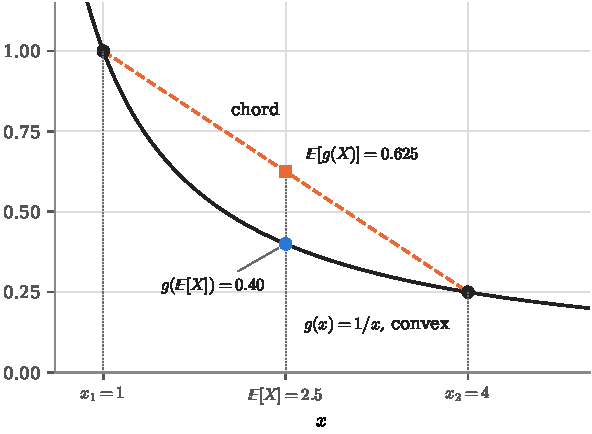
\includegraphics[width=0.7\textwidth]{fig_jensen}
\caption{Jensen's inequality for $g(x) = 1/x$ (solid curve) and an $X$ equal to $1$ or $4$ with probability $\frac12$ each. The orange dashed line is the chord; the blue dot is $(\E[X], g(\E[X]))$ and the orange square is $(\E[X], \E[g(X)])$.}
\label{fig:jensen}
\end{figure}

\begin{example}[The subway rate again]
In \cref{ch:limit-tools} the rate of the T was estimated by $\hat{\lambda} = 1/\bar{T}_n$, with $\E[\bar{T}_n] = 1/\lambda$.
Since $g(x) = 1/x$ is convex on $(0, \infty)$, Jensen gives $\E[1/\bar{T}_n] \geq 1/\E[\bar{T}_n] = \lambda$: the estimator is biased upward, for every $n$.
The bias does vanish as $n$ grows, but not because the estimator is consistent and asymptotically normal (neither property says anything about the bias); it vanishes because an exact computation gives $\E[1/\bar{T}_n] = \frac{n}{n-1}\lambda$, a bias of $\lambda/(n-1)$, which is of order $1/n$ and so is swamped by the $1/\sqrt{n}$ standard error. The exercises take this up.
Biased and consistent is a common combination, and nothing is wrong with it.
\end{example}

\begin{bridge}[why the sample variance divides by $n - 1$]
An introductory course divides the sum of squared deviations by $n - 1$, and the reason is a bias calculation.
For $\Xton$ i.i.d.\ with mean $\mu$ and variance $\sigma^2$, the natural estimator $\frac{1}{n} \sum (X_i - \bar{X}_n)^2$ has expectation
\[
\E \left[ \frac1n \sum_{i=1}^n (X_i - \bar{X}_n)^2 \right] = \E \left[ \frac1n \sum_{i=1}^n (X_i - \mu)^2 \right] - \E \left[ (\bar{X}_n - \mu)^2 \right] = \sigma^2 - \frac{\sigma^2}{n} = \frac{n-1}{n} \sigma^2,
\]
using $\sum (X_i - \bar{X}_n)^2 = \sum (X_i - \mu)^2 - n(\bar{X}_n - \mu)^2$.
Its bias is $-\sigma^2/n$: the deviations from $\bar{X}_n$ are systematically smaller than the deviations from $\mu$ because $\bar{X}_n$ was chosen to be in the middle of this sample.
Multiplying by $n/(n-1)$ removes the bias exactly, which is the $S^2 = \frac{1}{n-1} \sum (X_i - \bar{X}_n)^2$ you were taught.
Both versions are consistent; the correction matters at $n = 5$ and not at $n = 500$.
\end{bridge}

\section{Variance}
\label{sec:est-variance}

An estimator is a random variable, so it has a variance, $\var(\ethn) = \E[(\ethn - \E[\ethn])^2]$, which measures how widely it scatters around its own mean (not around $\theta$).
Small variance means the estimate you got is close to the estimate you would have got from a different sample; it says nothing about whether either is close to $\theta$.

\begin{worked}[four estimators of $p$: variance]
For the same four estimators, with $\var(X_i) = p(1-p)$:
\begin{enumerate}[nosep]
\item $\bar{X}_n$: $\var = p(1-p)/n$, since the variance of a sum of independent terms is the sum of the variances.
\item $X_1$: $\var = p(1-p)$. Unbiased, but as variable as a single coin flip, however large $n$ is.
\item $(X_1 + X_2)/2$: $\var = p(1-p)/2$.
\item $\sqrt{\ind(X_1 = 1, X_2 = 1)}$: a Bernoulli with parameter $p^2$, so $\var = p^2(1 - p^2)$.
\end{enumerate}
The first three are unbiased, so among them the comparison is purely on variance, and $\bar{X}_n$ wins by a factor of $n$ over $X_1$.
This is the sense in which using all the data matters: an unbiased estimator that ignores observations is paying in variance for no return in bias.
\Cref{fig:fourestimators} draws all four sampling distributions on one axis.
$\bar{X}_n$ is a narrow spike at $p$.
$X_1$ is two bars, at $0$ and $1$: unbiased, since its mean is $p$, and never anywhere near $p$.
$(X_1 + X_2)/2$ is three bars.
The square-root indicator is two bars with its mean at $p^2 = 0.42$, off the truth.
Bias is where the triangle sits relative to the orange line, variance is how spread out the bars are, and only the first estimator does well on both.
\end{worked}

\begin{figure}[htbp]
\centering
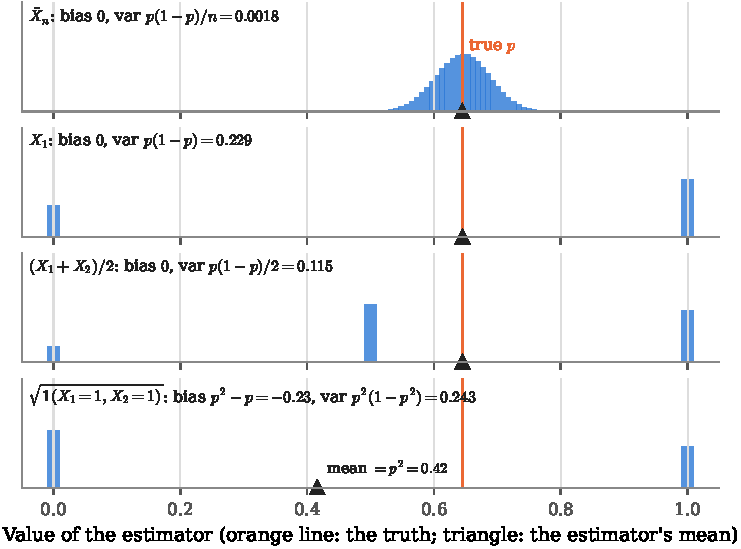
\includegraphics[width=\textwidth]{fig_four_estimators}
\caption{The exact sampling distributions (blue bars) of the four estimators of $p$ at $n = 124$, $p = 0.645$. The orange line is the true $p$; the black triangle under each axis is the estimator's mean.}
\label{fig:fourestimators}
\end{figure}

For the uniform example, $\var(\bar{X}_n) = \var(X_1)/n = \frac{1}{12n}$, and the bias-corrected $\bar{X}_n - \frac12$ has the same variance, since subtracting a constant changes nothing.

\section{Quadratic risk}
\label{sec:est-risk}

It may not be possible to find an estimator that is both unbiased and has the smallest variance.
Is there a compromise that can be made between a biased estimator and a high-variance one?
That is, can you find an estimator that simply has a small bias and a small variance?
That's where the quadratic risk comes in: a single number that charges for both.

\begin{definition}[Quadratic risk]
\label{def:risk}
The \textbf{quadratic risk} (or \textbf{risk}) of an estimator $\ethn \in \real$ is
\[
R(\ethn) = \E_\theta \left[ \abs{\ethn - \theta}^2 \right],
\]
the expected squared distance from the estimator to the truth.
It is more commonly called the \textbf{mean squared error}, and the two names mean the same thing.
\end{definition}

\begin{inwords}
\textbf{In words.} Square the miss, average over all possible samples. One number that punishes both a systematic lean and a wide scatter.
\par\smallskip
\textbf{For the kiss data.} $R(\bar{R}_n) = p(1-p)/n = 0.00185$ at $p = 0.645$, $n = 124$; a typical miss is its square root, $0.043$.
\end{inwords}

\begin{theorem}[Bias-variance decomposition]
\label{thm:bias-variance}
\[
R(\ethn) = \var(\ethn) + \Bias(\ethn)^2.
\]
\end{theorem}

\coreproof{Add and subtract $\E[\ethn]$ inside the square, expand, and watch the cross term vanish because $\E[\ethn - \E[\ethn]] = 0$.}
\begin{proof}
First note that $\abs{\ethn - \theta}^2 = (\ethn - \theta)^2$.
Add and subtract $\E[\ethn]$ inside the square and expand:
\begin{align*}
R(\ethn) &= \E\left[ ( \ethn - \E[\ethn] + \E[\ethn] - \theta)^2 \right] \\
	&= \E \left[ (\ethn  - \E[\ethn])^2 \right] + \E \left[ (\E[\ethn] - \theta)^2 \right] + 2 \E\left[(\ethn - \E[\ethn]) (\E[\ethn] - \theta) \right] \\
	&= \var(\ethn) + (\E[\ethn] - \theta)^2 + 2 (\E[\ethn] - \theta) \, \E\left[\ethn - \E[\ethn] \right] \\
	&= \var(\ethn) + \Bias(\ethn)^2 + 2 (\E[\ethn] - \theta) \cdot 0.
\end{align*}
In the second term, $\E[\ethn] - \theta$ is a number, so its expectation is itself; in the third, the same number comes out of the expectation, and what remains, $\E[\ethn - \E[\ethn]]$, is zero.
\end{proof}

\begin{bridge}[the MSE in an ANOVA table]
An introductory course's ANOVA table reports MSE, the mean square for error: the squared deviations of the observations from their group means, summed and divided by $N - k$ for $N$ observations in $k$ groups (simple regression output divides the sum of squared residuals by $N - 2$ instead).
It shares a name with the quadratic risk, but the squares it averages are residuals, not an estimator's misses.
MSE is a statistic, computed from the data, and an unbiased estimator of $\sigma^2$, the common variance of the model's errors.
The quadratic risk is an expectation under $\Pr_\theta$, a function of the unknown parameter, and no data set produces it.
The two meet in the standard error: with one group the MSE is the sample variance $S^2$, and $S^2/n$, the square of the estimated standard error $S/\sqrt{n}$, is an unbiased estimator of $\sigma^2/n$, which is the risk of $\bar{X}_n$ since $\bar{X}_n$ is unbiased.
\end{bridge}

The decomposition is the reason a biased estimator can be the better one: if accepting a little bias buys a large reduction in variance, the risk goes down.
It also makes a point that is easy to miss when you only ever compute bias and variance separately: the risk is a function of $\theta$, through both terms, and an estimator that is best for one value of $\theta$ need not be best for another.
\Cref{fig:biasvariance} shows both facts in the kiss model.
On the left, at $p = 0.645$ and $n = 124$, $\bar{R}_n$ is unbiased with standard deviation $0.043$.
The shrinkage estimator $(n\bar{R}_n + 10)/(n + 20)$ pulls the estimate toward $\frac12$, as if $20$ extra coin flips had come up half heads; it is biased by $-0.020$ but has standard deviation $0.037$, and its risk, $0.00177$, is smaller than $\bar{R}_n$'s $0.00185$.
On the right, the risk of four estimators is plotted against the true $p$.
Shrinkage beats $\bar{R}_n$ for $p$ between $0.34$ and $0.66$ and loses outside; the constant $0.5$ is unbeatable at $p = 0.5$ and terrible elsewhere; $X_1$ is unbiased and hopeless everywhere.
No curve lies below all the others, so `best estimator' is not a well-posed question without saying for which $p$.

\begin{figure}[htbp]
\centering
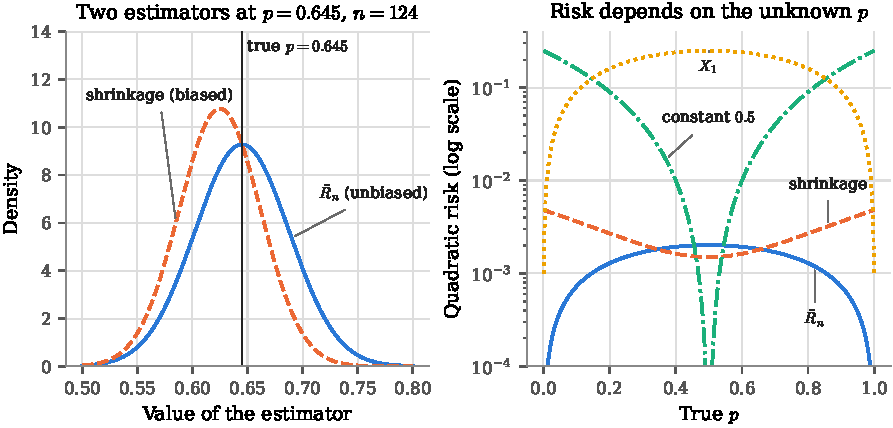
\includegraphics[width=\textwidth]{fig_bias_variance}
\caption{The kiss model, $n = 124$. Left: Gaussian approximations to the sampling distributions of $\bar{R}_n$ (solid) and the shrinkage estimator (dashed) at $p = 0.645$. Right: risk against the true $p$, log scale: $\bar{R}_n$ (solid), shrinkage (dashed), the constant $0.5$ (dash-dot), $X_1$ (dotted).}
\label{fig:biasvariance}
\end{figure}

\begin{intuition}[bias and variance as a target]
Think of the truth $\theta$ as the bull's-eye and each estimate as a shot.
Variance is how tight the group is; bias is how far the center of the group is from the bull's-eye.
The risk is the average squared distance of a shot from the bull's-eye, and the decomposition says it's the squared distance of the group's center plus the group's spread: a tight group off to one side can be closer on average than a loose group centered on the target.
The shrinkage estimator in \cref{fig:biasvariance} is the tight group off to one side.
What the target picture doesn't show is that moving the bull's-eye (changing $p$) changes which group is closer, and that's the right of \cref{fig:biasvariance}.
\Cref{fig:target} draws the four combinations.
The cross in each is $\E[\ethn]$, so bias is the distance from the cross to the bull's-eye, variance is the spread of the dots around the cross, and the risk is the average squared distance from a dot to the bull's-eye, which the decomposition splits into the two.
Lower left is the shrinkage estimator of \cref{fig:biasvariance}: a tight group slightly off center, closer on average than the loose group centered on the target at upper right.
\end{intuition}

\begin{figure}[htbp]
\centering
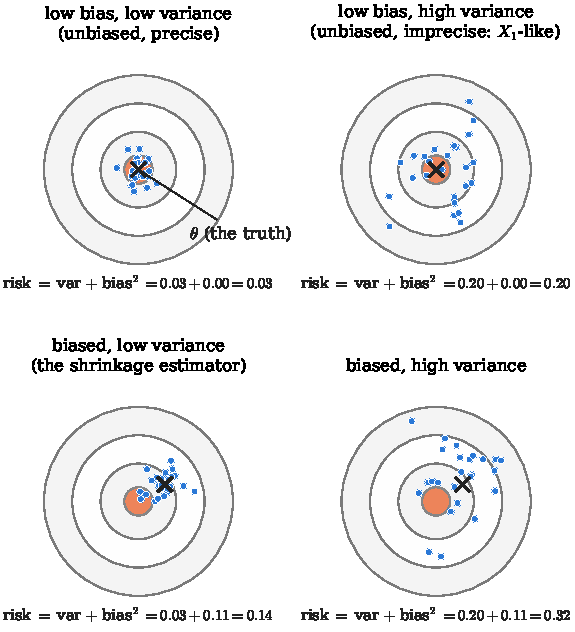
\includegraphics[width=0.78\textwidth]{fig_target}
\caption{Bias and variance as a target, in the four combinations. The bull's-eye is the truth $\theta$; each blue dot is the estimate from one sample; the black cross is the center of the group, $\E[\ethn]$.}
\label{fig:target}
\end{figure}

The target picture also settles a question the earlier bridge on $n - 1$ left open: Unbiased is not the same as closest.

\begin{bridge}[the $n - 1$ story, finished]
Among estimators of the form $c\sum_i (X_i - \bar{X}_n)^2$, the unbiased $S^2$ is not the one with the smallest quadratic risk.
For Gaussian data, dividing by $n + 1$ instead gives a biased estimator with strictly smaller quadratic risk than both the $n$ and $n - 1$ versions.
It is rarely used, since unbiasedness is a convention that makes results comparable across studies.
At $n = 12$ the risks are $0.182\sigma^4$, $0.160\sigma^4$ and $0.154\sigma^4$ for the divisors $n - 1$, $n$ and $n + 1$, and \cref{ex:t-nplus1} proves the general case.
\end{bridge}

\section{Strengths and weaknesses of estimators}
\label{sec:est-strengths}

Everything in this chapter can be applied at once to three estimators of $p$ for $\Xton \iid \Bern(p)$, $n$ large: $\bar{X}_n$, the constant $0.5$, and $X_1$.
Four criteria: bias, consistency, whether the estimator is efficiently computable (in this section, whether there is an explicit formula for it; the maximum likelihood estimators of \cref{ch:glm-links} have no closed form and are found by an iterative algorithm instead), and whether the quadratic risk tends to $0$ as $n \to \infty$.

\begin{center}
\small
\begin{tabular}{@{}l>{\raggedright\arraybackslash}p{1.1in}>{\raggedright\arraybackslash}p{1.1in}>{\raggedright\arraybackslash}p{1.1in}>{\raggedright\arraybackslash}p{1.3in}@{}}
\toprule
Estimator & Bias & Consistent? & Explicit formula? & Risk $\to 0$? \\
\midrule
$\bar{X}_n$ & $0$ & yes (LLN) & yes & yes: $p(1-p)/n$ \\[2pt]
$0.5$ & $0.5 - p$, nonzero unless $p = \frac12$ & no, unless $p = \frac12$ & yes & no: $(0.5 - p)^2$ for every $n$ \\[2pt]
$X_1$ & $0$ & no: it's $0$ or $1$, never near $p$ & yes & no: $p(1-p)$ for every $n$ \\
\bottomrule
\end{tabular}
\end{center}

The constant $0.5$ uses none of the data, so nothing can be learned from it; its only virtue is that it's exactly right when $p = \frac12$.
$X_1$ is unbiased, which sounds good, and uses one observation out of $n$, which is the actual problem: its risk doesn't shrink, so its accuracy is limited no matter how many samples are collected.
$\bar{X}_n$ has every property on the list.
Unbiasedness is desirable and may be the first thing to check, but the comparison with $X_1$ shows why it isn't enough: there are estimators that are unbiased and have a lot of variability, and risk is the number that catches them.

\begin{bridge}[random sampling for bias, a larger sample for variability]
An introductory course often draws the four targets of \cref{fig:target} with two rules: random sampling reduces bias, and a larger sample reduces variability.
The two rules act on the two terms of \cref{thm:bias-variance}.
Random sampling makes each $R_i$ a draw from $\Bern(p)$ with $p$ the population's proportion, which is all that $\E[\bar{R}_n] = p$ needs.
A design that over-represents part of the population draws from $\Bern(p')$ instead, with $p' \neq p$, so $\bar{R}_n$ is unbiased and consistent for $p'$, and as an estimator of $p$ it has
\[
R(\bar{R}_n) = \frac{p'(1 - p')}{n} + (p' - p)^2,
\]
of which a larger sample shrinks only the first term.
The 1936 \textit{Literary Digest} poll had about $2.4$ million returned ballots and predicted that Landon would beat Roosevelt $57\%$ to $43\%$; of the votes cast for the two, Roosevelt won $62\%$ (Freedman, Pisani and Purves, \textit{Statistics}).
With $p' = 0.43$ and $p = 0.62$ the first term is $1.0 \times 10^{-7}$, a standard deviation of $0.0003$, and the second is $0.036$: the risk was almost all bias, a miss of $19$ points.
\end{bridge}

\section{What comes next}
\label{sec:est-next}

Asymptotic normality hands you a sentence, `the error of $\ethn$ is approximately $\Gauss(0, \sigma^2/n)$', and the next two chapters are the two ways of using it.
\Cref{ch:confidence-intervals} turns it into a range of plausible values of $\theta$ with a guaranteed capture rate; \cref{ch:tests-foundations} turns it into a yes/no decision about $\theta$ with a guaranteed error rate.
Both need the quantiles of \cref{ch:gaussian} and the plug-in step of \cref{ch:limit-tools}, since $\sigma^2$ usually depends on $\theta$.

\section{Summary}
\label{sec:est-summary}

\begin{itemize}[nosep]
\item A statistic is a function of the data; an estimator of $\theta$ is a statistic whose formula doesn't involve $\theta$. Both are random variables. A statistic partitions the sample space and keeps one number per cell; a sufficient statistic keeps everything the sample says about $\theta$.
\item Consistent: $\ethn \convp \theta$ under $\Pr_\theta$, for every $\theta$. The sample mean is $\sqrt{n}$-consistent: its error is of exact order $1/\sqrt{n}$ (\cref{ex:rate}). Asymptotically normal: $\sqrt{n}(\ethn - \theta) \convd \Gauss(0, \sigma^2)$; $\sigma^2$ is the asymptotic variance, the variance of the limiting Gaussian, which for the sample mean equals $n \var(\bar{X}_n)$ and is never the limit of $\var(\ethn)$, which for any estimator whose variance shrinks is $0$ and carries no information.
\item Bias: $\E[\ethn] - \theta$. Unbiased means right on average. Convex or concave functions of unbiased estimators are biased, in the direction Jensen's inequality says: $g(\E[X]) \leq \E[g(X)]$ for convex $g$.
\item Variance: spread of $\ethn$ around its own mean. Using more of the data lowers it.
\item Quadratic risk: $\E[(\ethn - \theta)^2] = \var + \Bias^2$. It depends on $\theta$; a biased estimator can have lower risk than an unbiased one, and no estimator has the lowest risk for every $\theta$.
\item Of $\bar{X}_n$, the constant $\frac12$ and $X_1$, only $\bar{X}_n$ is unbiased, consistent and has risk tending to $0$. Unbiasedness alone, as $X_1$ shows, is not enough.
\end{itemize}

\section{Exercises}
\label{sec:est-exercises}

\begin{exercise}
Let $\Xton \iid \text{Unif}([a, a+1])$. Find $\E[\bar{X}_n]$, the bias of $\bar{X}_n$ for $a$, $\var(\bar{X}_n)$, and the quadratic risk of $\bar{X}_n - \frac12$.
\end{exercise}
\begin{solution}
$\E[\bar{X}_n] = a + \frac12$, bias $\frac12$. $\var(X_1) = \int_a^{a+1} x^2 \, \mathrm{d}x - (a + \frac12)^2 = a^2 + a + \frac13 - a^2 - a - \frac14 = \frac{1}{12}$, so $\var(\bar{X}_n) = \frac{1}{12n}$. The estimator $\bar{X}_n - \frac12$ is unbiased with the same variance, so its risk is $\frac{1}{12n}$, which tends to $0$.
\end{solution}

\begin{exercise}
Let $\Xton \iid \Bern(p)$ and $\hat{p} = \sqrt{\ind(X_1 = 1, X_2 = 1)}$. Find its bias, variance and quadratic risk, and say whether it is consistent.
\end{exercise}
\begin{solution}
$\hat{p} \sim \Bern(p^2)$, so bias $= p^2 - p$, variance $= p^2(1-p^2)$, and risk $= p^2(1-p^2) + (p^2 - p)^2 = p^2(1 - p^2) + p^2(1-p)^2$. None of these depend on $n$, so the risk does not go to $0$. The estimator is not consistent either, for the direct reason that its distribution never changes with $n$: $\Pr(\abs{\hat{p} - p} > \epsilon)$ is the same positive number for every $n$. It never uses $X_3, \ldots, X_n$.
\end{solution}

\begin{exercise}
In the kiss model with $n = 124$, compute the bias, variance and risk of the shrinkage estimator $\tilde{p}_n = (n \bar{R}_n + 10)/(n + 20)$ at $p = 0.645$ and at $p = 0.9$, and compare each with $\bar{R}_n$.
\end{exercise}
\begin{solution}
$\E[\tilde{p}_n] = (np + 10)/(n + 20)$ and $\var(\tilde{p}_n) = n p(1-p)/(n+20)^2$. At $p = 0.645$: mean $0.6249$, bias $-0.0201$, variance $0.001369$, risk $0.001775$, against $\bar{R}_n$'s risk $0.001847$. At $p = 0.9$: mean $0.8444$, bias $-0.0556$, variance $0.000538$, risk $0.003625$, against $\bar{R}_n$'s $0.000726$. Shrinking toward $\frac12$ pays when $p$ is near $\frac12$ and costs five times over when it isn't; \cref{fig:biasvariance} shows the crossover at $p \approx 0.34$ and $0.66$.
\end{solution}

\begin{exercise}
Let $\Xton \iid \Expo(\lambda)$ and $\hat{\lambda} = 1/\bar{X}_n$. Use Jensen's inequality to determine the sign of the bias, and use the fact (which you may take as given) that $\bar{X}_n$ has the Gamma distribution with $\E[1/\bar{X}_n] = \frac{n}{n-1} \lambda$ for $n \geq 2$ to find the bias exactly. Is there an unbiased estimator of $\lambda$ of the form $c/\bar{X}_n$?
\end{exercise}
\begin{solution}
$g(x) = 1/x$ is convex on $(0,\infty)$, so $\E[1/\bar{X}_n] \geq 1/\E[\bar{X}_n] = \lambda$: the bias is non-negative. Exactly, the bias is $\frac{n}{n-1}\lambda - \lambda = \frac{\lambda}{n-1}$, positive and of order $1/n$. The estimator $\frac{n-1}{n} \cdot \frac{1}{\bar{X}_n} = (n-1)/\sum X_i$ is unbiased.
\end{solution}

\begin{exercise}
Show that an estimator whose bias and variance both tend to $0$ is consistent. Is the converse true?
\end{exercise}
\begin{solution}
Bias and variance tending to $0$ means $R(\ethn) = \E[(\ethn - \theta)^2] \to 0$, which implies convergence in probability by Chebyshev's inequality (\cref{prop:shrinking-variance}; in the language of \cref{app:modes}, convergence in quadratic mean implies convergence in probability). The converse fails: convergence in probability does not require any moments to exist. For an example, take $\ethn = \theta$ with probability $1 - 1/n$ and $\ethn = n$ with probability $1/n$; then $\ethn \convp \theta$, but $\E[\ethn] = \theta(1 - 1/n) + 1 \to \theta + 1$, so the bias tends to $1$, not $0$.
\end{solution}
